% =====================================================================
%  Introduction to Deep Learning — Class 10
%  Topic (course plan): Deep Networks
%  Subtopics (course plan): Depth and Width efficiency, Theorems
%  Sources (course plan): Bishop Chapter 6, Prince Chapter 4, publications
%
%  Sequel to Class 9.  Class 9 settles what a network CAN represent and
%  at what rate; this class settles how the parameter budget should be
%  SPENT.  Nothing is repeated: the sawtooth, Telgarsky, Eldan-Shamir,
%  Montufar, Serra and the VC bound all live here, not in Class 9.
%
%  Figures: generated by src/build_all.py (one module per figure).
%  Notation: the fixed course convention (see _shared/NOTATION.md).
%
%  Compile:  xelatex main.tex   (run twice)
% =====================================================================
\documentclass[aspectratio=169, 11pt]{beamer}

\usetheme{metropoliscustom}

\usepackage{graphicx}
\DeclareGraphicsExtensions{.pdf,.png,.jpg}
\graphicspath{{figs/}{Class10_Depth_Width_Efficiency_Theorems/B_Recreated_Figures/figs/}}
\usepackage{amsmath, amssymb}
\usepackage{bm}
\usepackage{tikz}
\usetikzlibrary{arrows.meta, positioning, calc, decorations.pathreplacing}
\tcbuselibrary{skins}

\definecolor{shc}{HTML}{341651}
\definecolor{tealc}{HTML}{1C7293}
\definecolor{dpc}{HTML}{800000}
\definecolor{accc}{HTML}{B8860B}

% ---- theorem environments -------------------------------------------
\setbeamertemplate{theorems}[numbered]
\newtheorem{lemmax}[theorem]{Lemma}
\newtheorem{propx}[theorem]{Proposition}
\newtheorem{corx}[theorem]{Corollary}

% ---- parallel strip: Shallow (left) vs Deep (right) ------------------
\newcommand{\shpar}[2]{%
  \vfill
  {\scriptsize
  \begin{tcolorbox}[enhanced, sidebyside, sidebyside align=top,
                    lefthand ratio=0.485,
                    segmentation style={shc!35, line width=0.6pt},
                    colback=shc!5, colframe=shc!35, boxrule=0.5pt,
                    arc=1.2mm, left=1.6mm, right=1.6mm,
                    top=0.6mm, bottom=0.6mm,
                    before skip=0pt, after skip=0pt]
    {\color{shc}\textbf{SHALLOW}}\hspace{0.55em}#1
  \tcblower
    {\color{dpc}\textbf{DEEP}}\hspace{0.55em}#2
  \end{tcolorbox}}%
  \vspace{0.35em}%
}

\newcommand{\bridge}[1]{%
  {\scriptsize\itshape\color{mcMuted} #1\par}\vspace{0.35em}}

\newcommand{\figsource}[1]{{\scriptsize\color{mcMuted} #1}}
\newcommand{\figcap}[2][0.90]{%
  \begin{center}\begin{minipage}{#1\textwidth}\centering
    {\scriptsize\color{mcMuted} #2}
  \end{minipage}\end{center}}

\newcommand{\unit}[4]{%
  \node[circle, draw=#3, fill=#3!6, line width=0.7pt,
        minimum size=10mm, inner sep=0pt] (#1) at #2 {};
  \begin{scope}
    \clip #2 circle (0.5);
    \draw[tealc, line width=1.1pt]
      ($#2+(-0.50,-0.26)$) -- ($#2+(0.02,-0.26)$) -- ($#2+(0.46,0.28)$);
  \end{scope}
  \node[font=\large, #3] at ($#2+(0,0.78)$) {#4};
}
\newcommand{\plainunit}[4]{%
  \node[circle, draw=#3, fill=black!4, line width=0.7pt,
        minimum size=10mm, inner sep=0pt, font=\small] (#1) at #2 {#4};
}

% =====================================================================
\title{Deep Networks}
\subtitle{Depth and Width Efficiency, Theorems}
\author{Introduction to Deep Learning \ \textperiodcentered\ Class 10}
\institute{}
\date{}

\footleft{Introduction to Deep Learning}
\footright{Depth and Width Efficiency}
\titlelogos{}

\begin{document}

\maketitle

\begin{frame}{Outline}
  \tableofcontents
\end{frame}

% =====================================================================
\section{The Question Class 9 Left Open}
% =====================================================================

\begin{frame}{Where Class 9 left us}
  \vspace{0.2em}
  \begin{itemize}\setlength{\itemsep}{4pt}
    \item A tiling of fixed features costs $S^{D}$ parameters --- the
          \alert{curse of dimensionality}
    \item One hidden layer is already \alert{universal}, for any
          non-polynomial activation
    \item Rates: $O(C_f/\sqrt{M})$ on the Barron class, but
          $W^{-s/D}$ is unbeatable on a smoothness ball
    \item \alert{Width is a threshold}: at most $D+4$ units per layer
          is ever needed, and $\leq D$ never suffices
  \end{itemize}
  \vspace{0.4em}
  \begin{redhighlight}
    Every one of those results treats the network as a \emph{bag of
    parameters}. None of them asks how the budget should be
    \alert{shaped}.
  \end{redhighlight}
\end{frame}

\begin{frame}{Today's question, in one line}
  \vspace{-0.05em}
  \begin{center}
    {\large Given $W$ parameters, is it better to spend them on
    \alert{depth} or on \alert{width}?}
  \end{center}
  \vspace{0.15em}
  \centering
  \renewcommand{\arraystretch}{1.35}
  {\small
  \begin{tabular}{p{0.05\textwidth} p{0.42\textwidth}
                  p{0.40\textwidth}}
    & \textbf{Question} & \textbf{Answered by}\\
    \hline
    1 & What does it cost to replace depth with width?
      & Telgarsky; Liang \& Srikant; Eldan \& Shamir; Cohen;
        Safran \hfill{\scriptsize \S2}\\
    2 & What does it cost to replace width with depth?
      & Lu et al.; Vardi et al. \hfill{\scriptsize \S3}\\
    3 & How do we measure the power we are buying?
      & Mont\'ufar; Serra et al.; Bartlett et al.
        \hfill{\scriptsize \S4}\\
    4 & Why do these bounds not doom us in practice?
      & Poggio et al. \hfill{\scriptsize \S5}\\
    \hline
  \end{tabular}}
\end{frame}

% =====================================================================
\section{The Cost of Replacing Depth by Width}
% =====================================================================

\begin{frame}{A function built for the purpose}
  \bridge{To compare depth against width we need a target on which they
  can be told apart. One function does the whole job.}
  \vspace{0.3em}
  \begin{lemmax}[The sawtooth]
    {\small Let $T(x)=2h(x)-4h(x-\tfrac12)$ with $h=\mathrm{ReLU}$: a
    \alert{two-unit} network that maps $[0,1]$ onto $[0,1]$, folding it
    in half. Then $T^{\circ L}$ is piecewise linear with exactly
    $2^{L}$ pieces, and is computed by a network of depth $L$ and
    width $2$.}
  \end{lemmax}
  \vspace{0.2em}
  {\footnotesize
  \begin{itemize}\setlength{\itemsep}{1pt}
    \item \focus{1}{$T(x)=2x$ on $[0,\tfrac12]$ and $2-2x$ on
          $[\tfrac12,1]$: each half is mapped \alert{affinely onto all
          of} $[0,1]$}
    \item \focus{2}{\textbf{Base case.} $T^{\circ 1}$ has $2$ pieces}
    \item \focus{3}{\textbf{Induction.} $T^{\circ L}=T^{\circ(L-1)}
          \circ T$; on each half $T$ is affine and onto, so
          $T^{\circ L}$ restricted there is a rescaled copy of
          $T^{\circ(L-1)}$}
    \item \focus{4}{Two halves give $2\cdot 2^{L-1}=2^{L}$
          \hfill $\square$}
  \end{itemize}}
\end{frame}

\begin{frame}{Depth beats width, provably}
  \bridge{Every layer doubles the pieces. A single layer can only add
  them --- and that is already the whole separation.}
  \vspace{0.3em}
  \begin{theorem}[Depth--width separation; Telgarsky, 2016]
    {\small $T^{\circ L}$ is computed by a ReLU network with $O(L)$
    parameters, but any \alert{one-hidden-layer} ReLU network computing
    it exactly needs at least $2^{L}-1$ units. Telgarsky's published
    form is stronger: for every $k$ there are networks of $O(k^{3})$
    layers and constant width that no network of $O(k)$ layers can match
    with fewer than $2^{k}$ units.}
  \end{theorem}
  \vspace{0.3em}
  {\small
  \emph{Proof of the elementary form.} A one-hidden-layer ReLU network
  with $M$ units on a scalar input is piecewise linear with at most
  $M+1$ pieces (Class 5). Matching $2^{L}$ pieces forces
  $M+1\geq 2^{L}$. \hfill$\square$}
\end{frame}

\begin{frame}{The separation, measured}
  \vspace{-0.6em}
  \begin{center}
    
\includegraphics[height=0.735\textheight]{depth_width}
  \end{center}
\end{frame}

\begin{frame}{The cost of flattening}
  \bridge{The same two numbers, plotted against each other.}
  \vspace{-0.2em}
  \begin{center}
    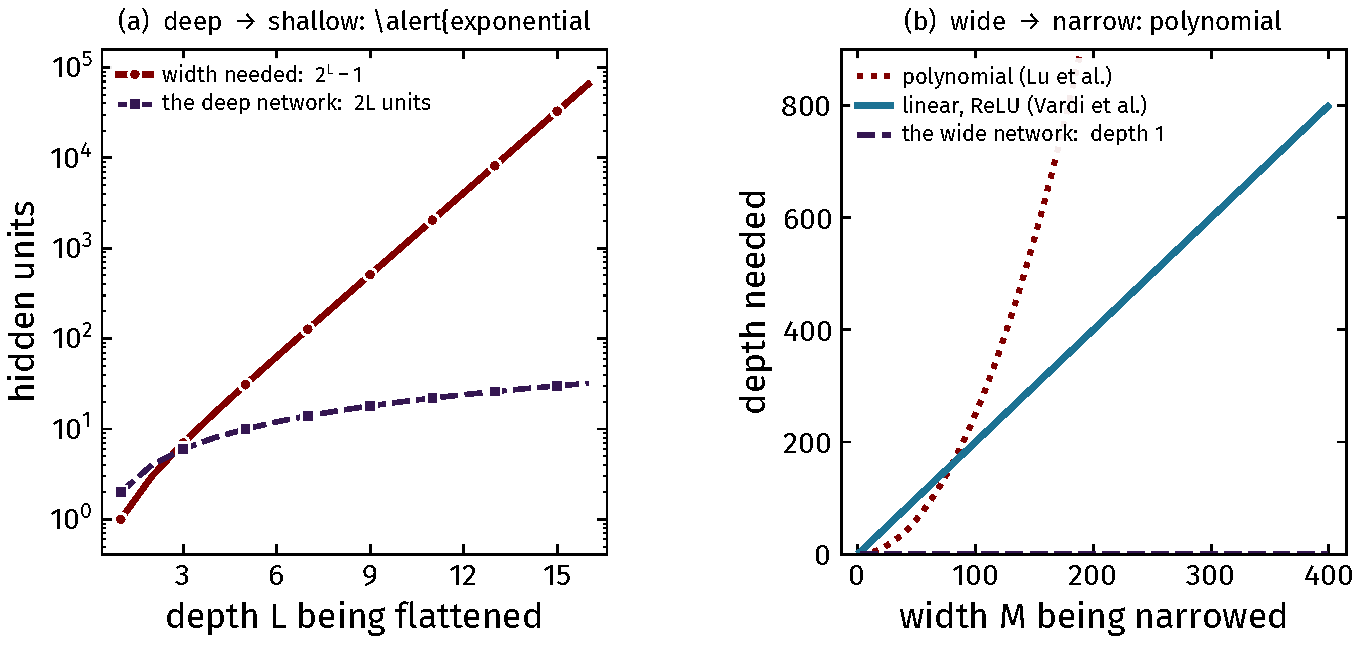
\includegraphics[height=0.47\textheight]{depth_width_asymmetry}
  \end{center}
  \figcap[0.96]{(a) flattening a depth-$L$ network of width 2 costs
  $2^{L}-1$ units against the $2L$ it had. (b) the reverse direction,
  \S3. Constants in (b) are illustrative; only the growth rates are
  claimed.}
\end{frame}

\begin{frame}{Not just one contrived function}
  \bridge{A sceptic will say the sawtooth was built to be hard. Three
  results say the phenomenon is generic.}
  \vspace{0.3em}
  \begin{theorem}[Liang \& Srikant, 2016]
    {\small For a broad class of functions --- including all
    sufficiently smooth univariate functions --- a shallow network needs
    \alert{exponentially more} hidden units than a deep one to reach the
    same approximation error.}
  \end{theorem}
  \vspace{0.4em}
  {\small
  \begin{itemize}\setlength{\itemsep}{4pt}
    \item The mechanism is the one we have already seen: deep networks
          build $x^{2}$, hence products, hence local polynomials,
          using $O(\log(1/\varepsilon))$ layers
    \item So the separation is not a property of one adversarial
          target but of a \alert{whole function class}
  \end{itemize}}
\end{frame}

\begin{frame}{A separation that grows with the dimension}
  \bridge{The sawtooth lives on a line. In many dimensions the gap
  appears for a different, and very natural, reason.}
  \vspace{0.3em}
  \begin{theorem}[Eldan \& Shamir, 2016]
    {\small There is a \alert{radial} function
    $g:\mathbb{R}^{D}\to\mathbb{R}$, supported on a ball, that a
    \alert{three-layer} network of $\mathrm{poly}(D)$ width approximates
    to within a constant in $L^{2}$, but which \alert{every two-layer}
    network needs width $\exp(\Omega(D))$ to approximate that well.}
  \end{theorem}
  \vspace{0.3em}
  {\small
  \begin{itemize}\setlength{\itemsep}{1pt}
    \item A two-layer network is a sum of \alert{ridge} functions, each
          constant along $D-1$ directions --- building a sphere out of
          hyperplanes is expensive
    \item Three layers first compute
          $\lVert\mathbf{x}\rVert^{2}=\sum_i x_i^{2}$ with $D$ cheap
          units, then apply a one-dimensional function to it
    \item Here the gap grows with the \alert{dimension}, not the depth
  \end{itemize}}
\end{frame}

\begin{frame}{And for almost every function}
  \bridge{Eldan--Shamir exhibits one hard function. The next result says
  the hard ones are the rule, not the exception.}
  \vspace{0.3em}
  \begin{theorem}[Cohen, Sharir \& Shashua, 2016]
    {\small Analysing networks through their \alert{tensor
    decomposition}: of the functions realisable by a deep network of
    polynomial size, the set that a shallow network can also realise
    (or even approximate) with polynomial size has
    \alert{measure zero}.}
  \end{theorem}
  \vspace{0.4em}
  {\small
  \begin{itemize}\setlength{\itemsep}{1pt}
    \item ``Almost all'' is meant literally --- in the measure-theoretic
          sense over the deep network's weights
    \item Proved for arithmetic circuits, where a network's function
          corresponds to a \alert{tensor}, and depth corresponds to its
          decomposition rank
    \item Complements Telgarsky: not one witness, but a full-measure
          set of them
  \end{itemize}}
\end{frame}

\begin{frame}{Even for a function you could draw}
  \bridge{One last witness, and the simplest of the four.}
  \vspace{0.4em}
  \begin{theorem}[Safran \& Shamir, 2017]
    {\small The indicator of the unit ball in $\mathbb{R}^{D}$ ---
    and simple radial functions like it --- is approximable in $L^{2}$
    to accuracy $\varepsilon$ by a \alert{three-layer} network of width
    $\mathrm{poly}(D,1/\varepsilon)$, but requires width
    $\exp(\Omega(D))$ for any \alert{two-layer} network.}
  \end{theorem}
  \vspace{0.5em}
  \begin{redhighlight}
    {\small Four independent constructions, three different mechanisms:
    folding, radial symmetry and tensor rank. \alert{Replacing depth by
    width is exponentially expensive.}}
  \end{redhighlight}
\end{frame}

% =====================================================================
\section{The Cost of Replacing Width by Depth}
% =====================================================================

\begin{frame}{The question, turned around}
  \bridge{We have only asked one of the two directions. The mirror
  question has a strikingly different answer.}
  \vspace{0.5em}
  \begin{center}
    {\large Is there a \alert{wide, shallow} network that a
    \alert{narrow, deep} one cannot reproduce cheaply?}
  \end{center}
  \vspace{0.6em}
  {\small
  \begin{itemize}\setlength{\itemsep}{4pt}
    \item Class 9 gave the existence half: width $D+4$ with enough
          depth is universal, and width $\leq D$ never is
    \item That says a narrow deep network \emph{can} do the job. It
          says nothing about \alert{how much depth} it costs
  \end{itemize}}
  \shpar{cheap to make wide}
        {cheap to make deep --- but are the two symmetric?}
\end{frame}

\begin{frame}{Width efficiency}
  \vspace{0.3em}
  \begin{theorem}[Width efficiency; Lu, Pu, Wang, Hu \& Wang, 2017]
    {\small There exist classes of wide, shallow networks that can only
    be expressed by narrow networks whose depth is
    \alert{polynomial} in the width being replaced.}
  \end{theorem}
  \vspace{0.4em}
  \begin{theorem}[Vardi, Yehudai \& Shamir, 2022]
    {\small For ReLU networks the price of making the width small is
    only a \alert{linear} increase in depth.}
  \end{theorem}
  \vspace{0.5em}
  {\small
  \begin{itemize}\setlength{\itemsep}{3pt}
    \item So narrowing a network is cheap: pay linearly in depth
    \item Flattening one is not: pay \alert{exponentially} in width
  \end{itemize}}
\end{frame}

\begin{frame}{The asymmetry, and what it decides}
  \vspace{0.05em}
  \centering
  \renewcommand{\arraystretch}{1.4}
  {\small
  \begin{tabular}{p{0.30\textwidth} p{0.28\textwidth}
                  p{0.32\textwidth}}
    & \textbf{\color{dpc}Remove depth}
    & \textbf{\color{shc}Remove width}\\
    \hline
    What you must add & width & depth\\
    How much & \alert{exponential} & \alert{polynomial}, and for ReLU
                                     \alert{linear}\\
    Established by & Telgarsky; Eldan \& Shamir; Cohen; Safran
                   & Lu et al.; Vardi et al.\\
    \hline
  \end{tabular}}
  \vspace{0.05em}
  \begin{redhighlight}
    The lower bound on width is \alert{exponential}; the lower bound on
    depth is only \alert{polynomial}. The two resources are not
    interchangeable --- \alert{depth is the more valuable one.}
  \end{redhighlight}
\end{frame}

% =====================================================================
\section{Measuring the Power Being Bought}
% =====================================================================

\begin{frame}{Counting linear regions}
  \bridge{Separations compare two architectures on one function. A
  region count measures an architecture on its own.}
  \vspace{0.3em}
  \begin{theorem}[Lower bound; Mont\'ufar, Pascanu, Cho \& Bengio, 2014]
    {\small A ReLU network with $L$ hidden layers of width $M\geq D$ on
    $\mathbb{R}^{D}$ can realise at least
    \[
      \Big(\prod_{l=1}^{L-1}\big\lfloor M/D \big\rfloor^{D}\Big)
      \sum_{j=0}^{D}\binom{M}{j}
    \]
    linear regions.}
  \end{theorem}
  \vspace{0.3em}
  {\small The trailing $\sum_{j\leq D}\binom{M}{j}$ is the
  \alert{Zaslavsky count} from Class 5: the last layer behaves like a
  shallow network, and the product in front is what depth adds.}
\end{frame}

\begin{frame}{Counting linear regions: the ceiling}
  \vspace{0.3em}
  \begin{theorem}[Upper bound; Serra, Tjandraatmadja \& Ramalingam, 2018]
    {\small The number of regions is at most
    $\prod_{l=1}^{L}\sum_{j=0}^{D}\binom{M}{j}$, and tighter bounds
    follow from the dimensions of the individual layers. The same
    authors give an algorithm that counts the regions of a trained
    network exactly.}
  \end{theorem}
  \vspace{0.5em}
  {\small
  \begin{itemize}\setlength{\itemsep}{4pt}
    \item Both bounds are \alert{exponential in $L$} and only
          \alert{polynomial in $M$} --- the same asymmetry as \S2--3,
          arrived at by a different route
    \item A lower bound says such networks \alert{exist}; it does not
          say training finds them
  \end{itemize}}
\end{frame}

\begin{frame}{Regions against parameters}
  \begin{center}
    
\includegraphics[height=0.505\textheight]{regions_bounds}
  \end{center}
  \figcap[0.96]{Regions against the parameter count $W$, for (a) a
  scalar input and (b) $D=5$. Grey is the shallow count; the coloured
  curves are the Mont\'ufar lower bound at three depths; dotted is the
  product upper bound at $L=3$. Widths are taken in multiples of $D$,
  where the lower bound is stated.}
\end{frame}

\begin{frame}{Capacity has a price}
  \bridge{Every result so far has been an argument for depth. Here is
  the bill.}
  \vspace{0.3em}
  \begin{theorem}[VC dimension; Bartlett, Harvey, Liaw \& Mehrabian, 2019]
    {\small For ReLU networks with $W$ parameters and $L$ layers,
    $\mathrm{VCdim} = \Theta\big(W L \log W\big)$.}
  \end{theorem}
  \vspace{0.4em}
  {\small
  \begin{itemize}\setlength{\itemsep}{3pt}
    \item Learning theory then needs
          $N=\Omega(\mathrm{VCdim}/\epsilon^{2})$ samples for a
          generalisation gap $\epsilon$
    \item Modern networks have $\mathrm{VCdim}\gg N$ and generalise
          anyway: the bound is \alert{loose} for real data (Class 17)
  \end{itemize}}
  \vspace{0.2em}
  \begin{redhighlight}
    {\small Expressivity and generalisation theorems pull in
    \alert{opposite directions}; neither alone explains deep learning.}
  \end{redhighlight}
\end{frame}

\begin{frame}{VC dimension, drawn}
  \begin{center}
    
\includegraphics[height=0.505\textheight]{vc_growth}
  \end{center}
  \figcap[0.96]{(a) $\Theta(WL\log W)$ against the parameter count, at
  four depths, with a linear reference. (b) at a fixed $W=10^{5}$, the
  worst-case number of samples the VC bound demands for a
  generalisation gap of $0.1$ --- growing linearly with depth.}
\end{frame}

% =====================================================================
\section{Why the Bounds Do Not Doom Us}
% =====================================================================

\begin{frame}{The tension to resolve}
  \vspace{0.3em}
  \begin{itemize}\setlength{\itemsep}{5pt}
    \item Class 9: on a smoothness ball, $W^{-s/D}$ is
          \alert{unbeatable} --- the curse is a theorem, not a
          pessimism
    \item Today: depth is exponentially more efficient than width ---
          but efficient \emph{relative} to shallow, which was already
          hopeless
    \item Yet networks with $10^{6}$ parameters routinely solve
          problems with $D=10^{6}$
  \end{itemize}
  \vspace{0.5em}
  \begin{redhighlight}
    Something about \alert{real targets} must be special. The last
    theorem of the lecture says what.
  \end{redhighlight}
\end{frame}

\begin{frame}{Compositional functions escape the curse}
  \vspace{0.2em}
  \begin{theorem}[Poggio, Mhaskar, Rosasco, Miranda \& Liao, 2017]
    {\small Let $f$ be \alert{compositional}: built from a binary tree
    of two-variable constituent functions, each of smoothness $m$. A
    deep network \emph{matching that tree} approximates $f$ to accuracy
    $\varepsilon$ with
    $O\big((D-1)\,\varepsilon^{-2/m}\big)$ parameters, whereas a
    shallow network needs $O\big(\varepsilon^{-D/m}\big)$.}
  \end{theorem}
  \vspace{0.4em}
  {\small
  \begin{itemize}\setlength{\itemsep}{3pt}
    \item The dimension moves out of the \alert{exponent} and into a
          \alert{linear factor} --- the curse is gone, for this class
    \item The deep network wins only when its \alert{architecture
          mirrors the target's structure}
    \item This is the formal version of the Class 7 slogan: strokes
          $\to$ letters $\to$ words $\to$ meaning
  \end{itemize}}
\end{frame}

\begin{frame}{The size of the effect}
  \begin{center}
    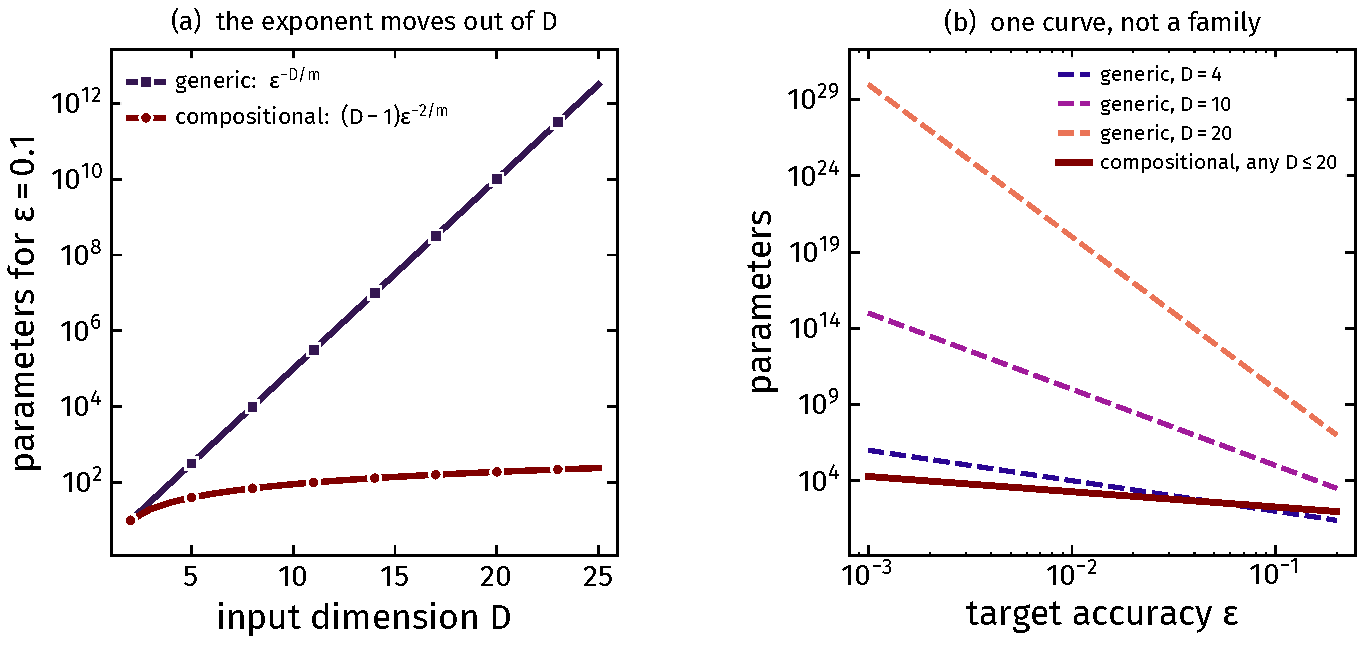
\includegraphics[height=0.50\textheight]{compositional}
  \end{center}
  \figcap[0.96]{(a) parameters needed for $\varepsilon=0.1$ against the
  input dimension: the generic bound climbs exponentially, the
  compositional one linearly. (b) the same against accuracy --- the
  generic bound is a family of curves indexed by $D$, the compositional
  bound is a single curve.}
\end{frame}

\begin{frame}{Why real data is compositional}
  \vspace{0.3em}
  \begin{itemize}\setlength{\itemsep}{5pt}
    \item An image label depends on \alert{local} structure first:
          pixels form edges, edges form parts, parts form objects ---
          exactly a tree of few-variable functions
    \item Language, audio and molecules have the same shape:
          short-range structure composed into long-range meaning
    \item Convolution hard-codes this tree; a fully connected network
          must \alert{learn} it, which is why architecture matters more
          than the parameter count suggests
  \end{itemize}
  \shpar{one flat map from $\mathbf{x}$ to $y$}
        {a tree of local maps --- matching how the data was generated}
\end{frame}

% =====================================================================
\section{Reading the Theorems}
% =====================================================================

\begin{frame}{What each result actually gives}
  \bridge{Nine results in one lecture. What each one is really
  claiming:}
  \vspace{-0.05em}
  \centering
  \renewcommand{\arraystretch}{1.2}
  {\scriptsize
  \begin{tabular}{p{0.235\textwidth} p{0.30\textwidth}
                  p{0.36\textwidth}}
    \textbf{Result} & \textbf{Gives} & \textbf{Does not give}\\
    \hline
    Telgarsky (2016)
      & an explicit exponential depth gap
      & that such functions arise in practice\\
    Eldan \& Shamir (2016)
      & a gap growing with $D$, at depth 3 vs 2
      & anything beyond three layers\\
    Cohen et al.\ (2016)
      & the gap holds for almost every deep function
      & a statement about ReLU MLPs directly\\
    Lu et al.\ (2017)
      & narrowing costs only polynomial depth
      & tight constants\\
    Vardi et al.\ (2022)
      & for ReLU, only linear depth
      & a matching lower bound\\
    Mont\'ufar / Serra
      & regions exponential in $L$
      & that training reaches them\\
    Bartlett et al.\ (2019)
      & $\mathrm{VCdim}=\Theta(WL\log W)$
      & a useful bound at modern scale\\
    Poggio et al.\ (2017)
      & the curse lifts for compositional targets
      & that a given target is compositional\\
    \hline
  \end{tabular}}
\end{frame}

\begin{frame}{What none of them say}
  \bridge{And the gap between all this and a working network:}
  \vspace{0.3em}
  \begin{itemize}\setlength{\itemsep}{5pt}
    \item \alert{Nothing about optimisation.} Every result is about the
          \emph{existence} of weights; finding them is Classes 11--14
    \item \alert{Nothing about generalisation.} The capacity bounds are
          worst-case over all data distributions
    \item \alert{The witnesses are constructed.} Sawtooths, radial
          bumps and tensor arguments are built to separate; natural
          signals are not adversarial
    \item \alert{Architecture beats arithmetic.} Poggio's result only
          bites when the network's shape matches the target's ---
          which is what convolution and attention are for
  \end{itemize}
\end{frame}

\begin{frame}{Takeaways}
  \vspace{0.1em}
  {\footnotesize
  \begin{enumerate}\setlength{\itemsep}{2pt}
    \item Depth and width are \alert{not interchangeable}. Replacing
          depth by width costs \alert{exponentially}; replacing width
          by depth costs only \alert{polynomially}, and for ReLU
          linearly
    \item The depth gap has been shown four ways --- folding
          (Telgarsky), a function class (Liang \& Srikant), radial
          symmetry (Eldan \& Shamir; Safran \& Shamir) and tensor rank
          (Cohen et al.) --- so it is \alert{not an artefact of one
          construction}
    \item Region counts reach the same asymmetry independently:
          exponential in $L$, polynomial in $M$
    \item The power is not free: $\mathrm{VCdim}=\Theta(WL\log W)$
          grows with depth too
    \item The curse lifts for \alert{compositional} targets, and only
          for a network whose \alert{architecture mirrors} the target's
          structure --- which is what real data looks like
  \end{enumerate}}
  \vspace{0.2em}
  \begin{redhighlight}
    {\footnotesize Class 11: we now know what to build. Next, how to
    \alert{train} it --- activations, error functions and
    backpropagation.}
  \end{redhighlight}
\end{frame}

\begin{frame}{References}
  \scriptsize
  \begin{itemize}\setlength{\itemsep}{1pt}
    \item S.~J.~D.~Prince. \textit{Understanding Deep Learning.}
          MIT Press, 2023. Ch.~4 and its notes on depth efficiency,
          width efficiency and the number of linear regions --- the
          source for this lecture's reading list.
    \item C.~M.~Bishop \& H.~Bishop. \textit{Deep Learning: Foundations
          and Concepts.} Springer, 2024. Ch.~6 --- hierarchical
          representations and the compositional inductive bias.
    \item M.~Telgarsky, \textit{COLT} (2016) --- benefits of depth.
    \item S.~Liang \& R.~Srikant, \textit{ICLR} (2017; arXiv 2016) ---
          why deep neural networks for function approximation.
    \item R.~Eldan \& O.~Shamir, \textit{COLT} (2016) --- the power of
          depth for feedforward neural networks.
    \item N.~Cohen, O.~Sharir \& A.~Shashua, \textit{COLT} (2016) ---
          on the expressive power of deep learning: a tensor analysis.
    \item I.~Safran \& O.~Shamir, \textit{ICML} (2017) --- depth
          separation in ReLU networks for approximating smooth
          non-linear functions.
  \end{itemize}
\end{frame}

\begin{frame}{References (continued)}
  \scriptsize
  \begin{itemize}\setlength{\itemsep}{1pt}
    \item Z.~Lu, H.~Pu, F.~Wang, Z.~Hu \& L.~Wang, \textit{NeurIPS}
          (2017) --- the expressive power of neural networks: a view
          from the width.
    \item G.~Vardi, G.~Yehudai \& O.~Shamir, \textit{COLT} (2022) ---
          width is less important than depth in ReLU networks.
    \item G.~Mont\'ufar, R.~Pascanu, K.~Cho \& Y.~Bengio,
          \textit{NeurIPS} (2014); T.~Serra, C.~Tjandraatmadja \&
          S.~Ramalingam, \textit{ICML} (2018) --- linear regions.
    \item P.~Bartlett, N.~Harvey, C.~Liaw \& A.~Mehrabian,
          \textit{JMLR} 20:63 (2019) --- VC dimension.
    \item T.~Poggio, H.~Mhaskar, L.~Rosasco, B.~Miranda \& Q.~Liao,
          \textit{Int.\ J.\ Autom.\ Comput.} 14:503 (2017) --- why and
          when deep but not shallow networks avoid the curse.
    \item Plots generated by \texttt{src/build\_all.py}.
  \end{itemize}
\end{frame}

\begin{frame}[standout]
  Questions?
\end{frame}

\end{document}
